\documentclass{school-22.101-notes}
\date{December 7, 2011}

\begin{document}
\maketitle

\topic{Fission}
Fission happens because braking a heavy nuclide into two smaller one is climbing up the B/A curve. 

Example: \ce{^{238}_{92}U \to 2 ^{119}_{49}Pd + (n, \beta, \gamma, KE) } 

We can calculate the energy release Q by doing parent binding energy minus daughter binding energy (most of these energy is carried by fission products): 
\eqn{ Q = 238 \times \underbrace{(-7.6 \fsp \MeV)}_{B/A \fsp \mathrm{U}} - 2 \times 119 \times \underbrace{(-8.5 \fsp \MeV)}_{B/A \fsp \mathrm{Pd}} = -1809 + 2023 = 214 \fsp \MeV  }

Recall spontaneous fission is not very common due to the Coulomb barrier; recall spontaneous fission has a long half-life: $t_{1/2}^{SF} = 10^16$ yr, $t_{1/2}^{\alpha} = 10^9$ yr. We assume the potential as the Coulomb barrier model, and based on $V^{\mathrm{peak}}$ vs Q graph three cases are possible as in Figure~\ref{fission-mechanism}:
\begin{enumerate}
\item $Q \sim V^{\mathrm{peak}}$: spontaneous fission, use Tunneling (some nuclei for which energy release puts the two fragments just below the Coulomb barrier, good probability to penetrate); 
\item $Q > V^{\mathrm{peak}}, A>300$: instantaneous spontaneous fission (some nuclei whose separated state would put tem alone the Coulomb barrier, not observed in nature);
\item $Q < V^{\mathrm{peak}}$: induced fission, provide help/energy to climb over the coulomb barrier, called Activation Energy (some nuclei energy releaste puts two fragments significantly below the Coulomb barrier; if some energy is given in, may be pushed over the barrier). 
\end{enumerate}
\begin{figure}[ht]
   \centering
   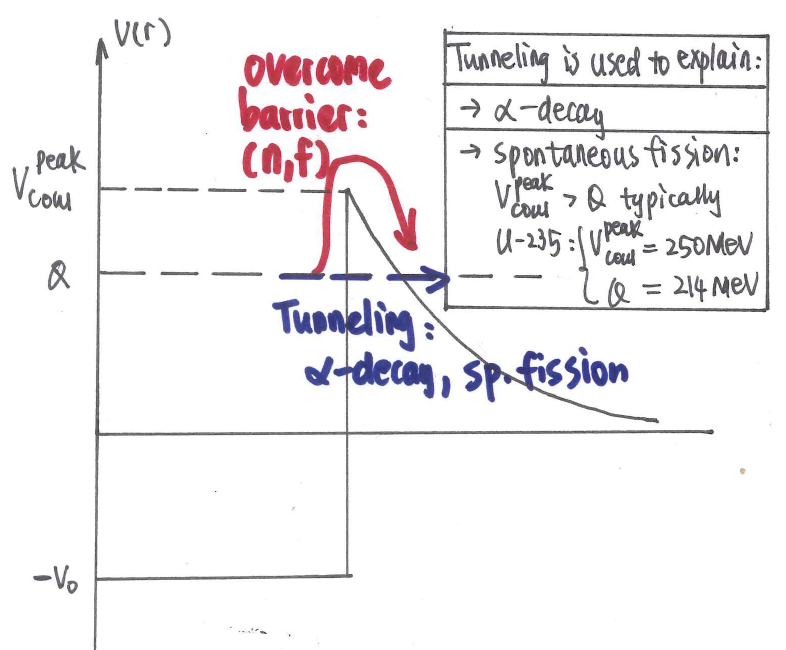
\includegraphics[width=3in]{images/ni/fission-mechanism.png}
   \caption{Mechanism to Overcome the Potential Barrier\label{fission-mechanism}}
\end{figure}

\subtopic{Induced Fission, Activation Energy}
The potential barrier the compound nucleus needs to overcome is called \textbf{Activation Energy for Fission} $E_{\mathrm{act}}$ as in Figure~\ref{activation-energy}. This may be a result from:
\begin{itemize}
\item KE of neutrons (esp. fast neutrons);
\item Mass of neutrons (esp. thermal neutrons);
\item Gamma energy (esp. photo-induced fission).
\end{itemize}
\begin{figure}
   \centering
   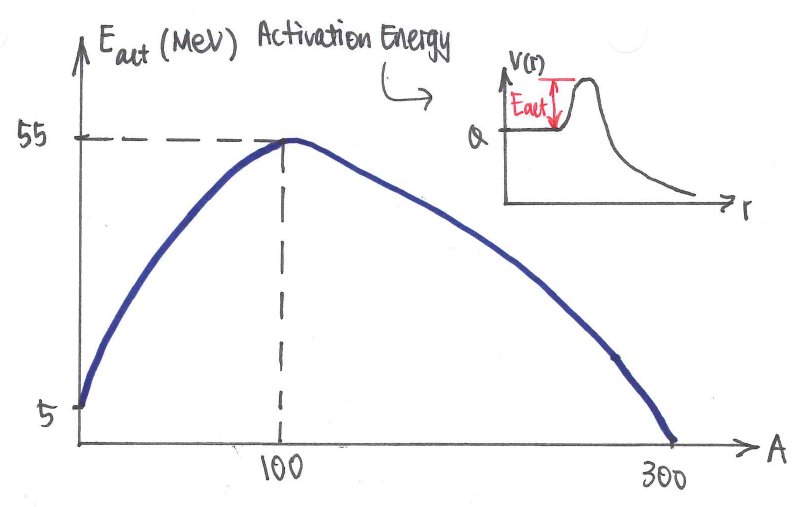
\includegraphics[width=4in]{images/ni/activation-energy.png}
   \caption{Activation Energy\label{activation-energy}}
\end{figure}
$Q$ can be calculated using SEMF, $E_{\mathrm{act}}$ can be calculated from Coulomb's law at the radius of interest (could be the sum of the radius of daughters or the radius of the parent nuclide). 

\begin{enumerate}
\item U235: \ce{ n + ^{235} U \to ^{236}U*}. Assume: neutron is thermal neutron with little/no KE; 
    \begin{enumerate}
    \item U236 compound energy is just the total rest mass energy of the reactants, 
    \eqn{ m(U236*) = m_n + m(U235) = 1.008665 u+ 235.043924u =236.052589u }
    \item U236 compound excitation energy is the difference between the compound energy and the group state energy:
    \eqn{ E_{\mathrm{ex}} = (m(U236*) - m(U236) ) c^2 = (236.052589u - 236.045563u) \times 931.5 \fsp \MeV/u = 6.54 \fsp \MeV}
    \item Whether this compound can induced fission depends on $E_{\mathrm{ex}}$ vs $E_{\mathrm{act}}$. We look up U236's activation energy $E_{\mathrm{act}}^{236} = 6.2 \fsp \MeV$, which is smaller than $E_{\mathrm{ex}}^{236*} = 6.5 \fsp \MeV$. That is to say, this compound can induce fission.
    \item Conclusion: thermal neutron can induce U235 to fission.  
    \end{enumerate}

\item U238: \ce{ n + ^{238} U \to ^{239}U*}. Assume: neutron is thermal neutron with little/no KE; 
    \begin{enumerate}
    \item U239 compound energy is just the total rest mass energy of the reactants,  
    \eqn{ m(U239*) = m_n + m(U238) = 1.008665 u+ 238.050785u =239.05945u}
    \item U239 compound excitation energy:
    \eqn{ E_{\mathrm{ex}} = (m(U239*) - m(U239) ) c^2= (239.05945-239.054290u)\times 931.5 \MeV/u  =4.8 \fsp \MeV}
    \item We look up U239's activation energy, $E_{\mathrm{act}}^{239} = 6.6 \fsp \MeV > E_{\mathrm{ex}}^{239*} = 4.8 \fsp \MeV$. That is to say, this compound can only induce fission with neutrons with KE more than $(6.6-4.8) \fsp \MeV = 1.8 \fsp \MeV$, which is fast neutrons.
    \item Conclusion: U-238 requires neutron with at least 1-2 MeV KE to induce fission.  
    \end{enumerate}

\item U235 compare with U238.
Paring effect see Figure~\ref{pairing-effect}. KE of incoming neutrons, see Figure~\ref{KE-incoming-neutron}. 
\begin{figure}
   \centering
   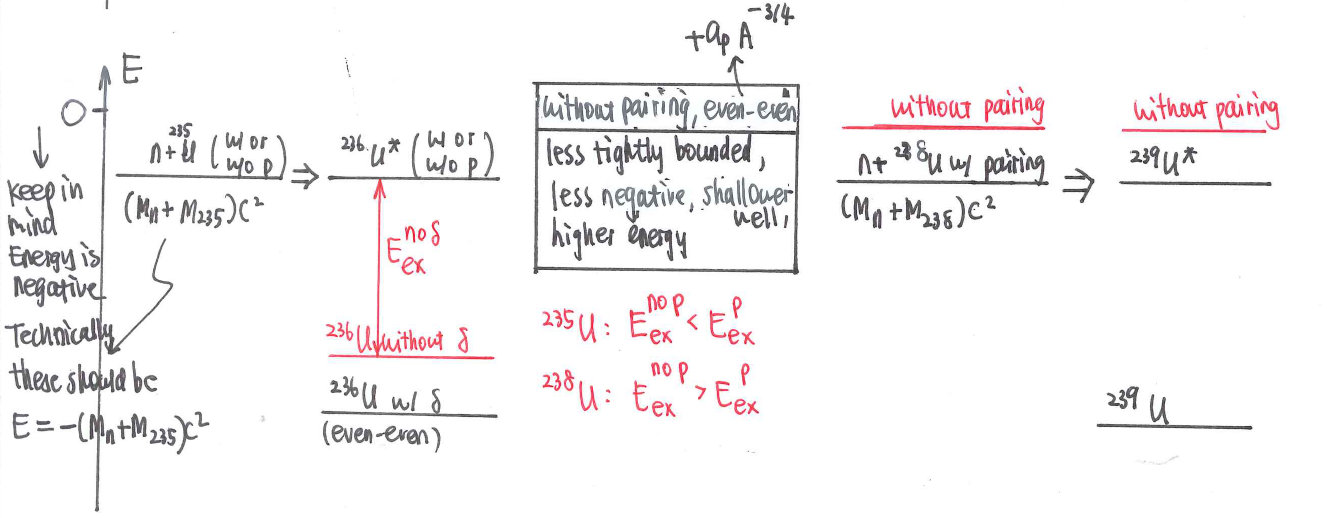
\includegraphics[width=6in]{images/ni/pairing-effect.png}
   \caption{Pairing Effect\label{pairing-effect}}
\end{figure}
\begin{figure}
   \centering
   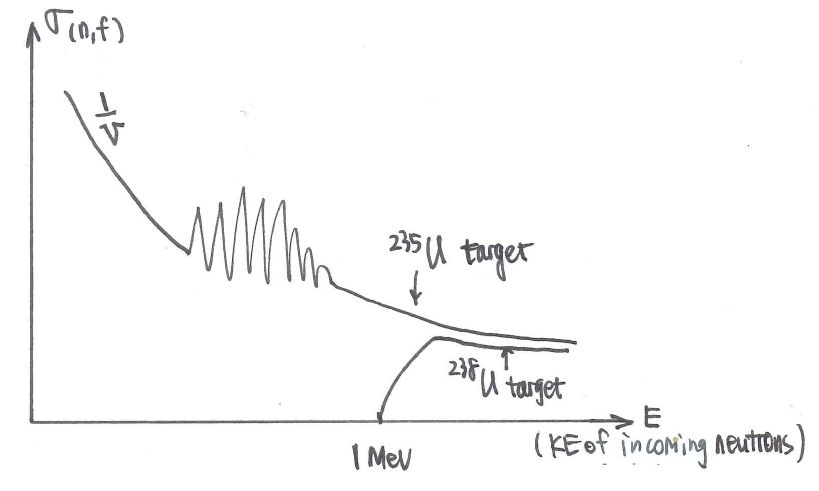
\includegraphics[width=4in]{images/ni/KE-incoming-neutron.png}
   \caption{KE of Incoming Neutron\label{KE-incoming-neutron}}
\end{figure}
\end{enumerate}

\topic{Fusion}
Fusion happens at $A<60$ on the B/A curve. Example: \ce{^{20}Ne + ^{20}Ne \to \ce{^{40}Ca}}, It turns out $Q = 20.7 \fsp \MeV < V^{\mathrm{peak}} = 21.2 \fsp \MeV$. To overcome the barrier, we need to:
\begin{itemize}
\item Increase thermal energy; not very practical because it has to be around $10^{11} K,$ from $\frac{3}{2} kT$. 
\item Accelerate ions to increase KE. $\eta \down, I \down \down 10^{-6} \sim 10^{-9} A, P \down$.
\end{itemize}

Basic Fusion Reactions: 
\begin{enumerate}
\item \ce{p + p \to \ce{^2He}} (not stable, reaction not possible); 
\item \ce{p + p \to \ce{^2H} + e^+ + \nu} (first step in solar fusion, analogus to beta decay);
\item \ce{^2 H + ^2 H \to \ce{^3He} + n}, Q = 3.3 MeV ($Q>0$, hence possible); 
\item \ce{^2 H + ^2 H \to \ce{^3H} + p}, Q = 4.0 MeV (probable);
\item \ce{^2H + ^3H \to \ce{^4He} + n}, Q = 17.6 MeV (probable, larger Q than D-D reaction, ideal choice).
\end{enumerate}
Notice $Q_{DD} < Q_{DT},$, would the potential barrier height is the same for both, hence D-T reaction is selected for use in controlled fusion. 

\subtopic{Energy Release}
How do we calculate the KE carried by the neutrons and protons? We use energy and momentum conservation, to figure out how much Q is carried by each of the daughter particles in the form of KE. It turns out the smaller the mass, the more KE it carries. 

\subtopic{Coulomb Barrier}
We need tunneling to penetrate through the potential barrier, now that we are incapable of getting rid of the barrier. Assume fusion reaction \ce{ a + X \to b + Y}. The Coulomb barrier we want to tunnel through is: 
\begin{align}
V_{\mathrm{coul}} &= \frac{Z_{a} Z_{X} e^2 }{R} \\
G &\sim \frac{Z_a Z_x}{\sqrt{Q}} \\
P_T &\sim e^{-2G} \sim e^{- \frac{Z_a Z_X}{\sqrt{Q}}} \\
\sigma_{\mathrm{fusion}} &\sim \frac{1}{v^2} P_T
\end{align}
in which Q is replaced by the sum of the KE of the nuclides before them merge, it is small, on the order of 10 keV; \textcolor{blue}{The smaller $Z_a Z_X$, the higher $P_T$.} 
\begin{figure}
   \centering
   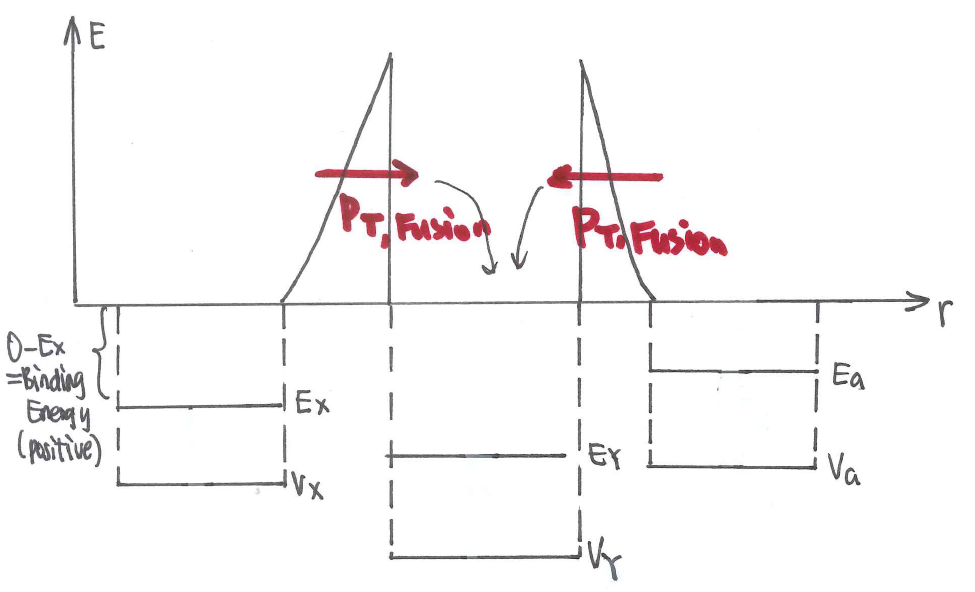
\includegraphics[width=4in]{images/ni/fusion-mechanism.png}
   \caption{Mechanism for Fusion\label{fusion-mechanism}}
\end{figure}



\end{document}
